\documentclass[11pt,a4paper]{article}
\usepackage{fontspec}
\usepackage{amsmath,amssymb,amsthm}
\usepackage{mathtools}
\usepackage{bm}
\usepackage{booktabs}
\usepackage{geometry}
\usepackage{enumitem}
\usepackage{graphicx}
\usepackage{xcolor}
\usepackage{tcolorbox}
\usepackage[pdfencoding=auto,psdextra]{hyperref}

\geometry{margin=2.5cm}

\newcommand{\E}{\mathbb{E}}
\newcommand{\R}{\mathbb{R}}
\newcommand{\KL}{\mathrm{KL}}
\newcommand{\N}{\mathcal{N}}
\newcommand{\Za}{\mathcal{Z}_{T}}
\newcommand{\Zb}{\mathcal{Z}_{S}}
\newcommand{\Enc}{\mathcal{E}}
\newcommand{\Dec}{\mathcal{D}}
\newcommand{\Bridge}{\mathcal{B}}
\newcommand{\Tmap}{\mathsf{T}}
\newcommand{\Tinv}{\mathsf{T}^{-1}}
\newcommand{\push}{\#}
\newcommand{\norm}[1]{\left\lVert #1 \right\rVert}

\theoremstyle{definition}
\newtheorem{remark}{Remark}
\newtheorem{observation}{Observation}

\title{\textbf{Cross-Space Distillation (Bridge)}\\[0.3em]
\large Mapping arXiv:2606.32020 onto XOPD's Cross-VAE Inverse Problem}
\author{Jayce-Ping}
\date{}

\begin{document}
\maketitle

\begin{abstract}
Companion note to \texttt{cross\_latent\_distillation\_problem.tex},
\texttt{avoid\_inverse\_transport\_analysis.tex}, and
\texttt{inverse\_mapping\_methods.tex}.
We summarize
\href{https://arxiv.org/abs/2606.32020}{Nguyen et~al., Cross-Space Distillation
(arXiv:2606.32020)} --- a method that trains a lightweight
\textbf{Bridge} $\Bridge_\phi:\Zb\to\Za$ so that compact one-step Students
(different resolution / VAE) can run standard distribution-based distillation
(VSD / GAN, DMD2-style) against modern Teachers.
Figures are taken from the arXiv e-print source (\texttt{assets/}).
The key mapping for our codebase: Bridge is a concrete construction of the
\emph{hard} student$\to$teacher inverse $Q$ (pixel-anchored spatial prior $+$
learned projector $+$ attention fidelity), but it is designed for
\emph{measure / score matching in Teacher space}, not for XOPD's pointwise
velocity pushforward L1. That places it closest to Route~A in the avoid-inverse
note, not to linear-$P$ L1 transport.
\end{abstract}

%% ============================================================
\section{Problem they formalize}
\label{sec:problem}
%% ============================================================

Distribution-based one-step distillation (VSD / adversarial / DMD-family) almost always
assumes a \textbf{Shared-Space} constraint: Teacher and Student share the same VAE and
latent grid, so Teacher scores / discriminators can be evaluated on Student samples
directly. Modern Teachers (SD~3.5, FLUX.2, \ldots at $1024^2$) and compact Students
(SD~1.5 / 2.1 at $512^2$) violate this in two coupled ways:

\begin{enumerate}[leftmargin=1.6em,itemsep=2pt]
  \item \textbf{Cross-Resolution:} $z_S\in\R^{h\times w\times C_S}$ vs.\
        $z_T\in\R^{H\times W\times C_T}$ with $(h,w)\neq(H,W)$.
  \item \textbf{Cross-VAE:} different autoencoders $\Rightarrow$
        $\Zb\not\cong\Za$ (channels, statistics, semantics).
\end{enumerate}

They call the joint regime \textbf{Cross-Space Distillation}. Empirically they argue that
cross-architecture (UNet vs.\ DiT) and cross-mechanism (DDPM vs.\ flow matching) are
secondary once outputs are reparameterized to a common $x_0$ estimate in a shared
(Teacher) latent; the \emph{blocking} mismatch is resolution $+$ VAE.

\begin{figure}[t]
\centering
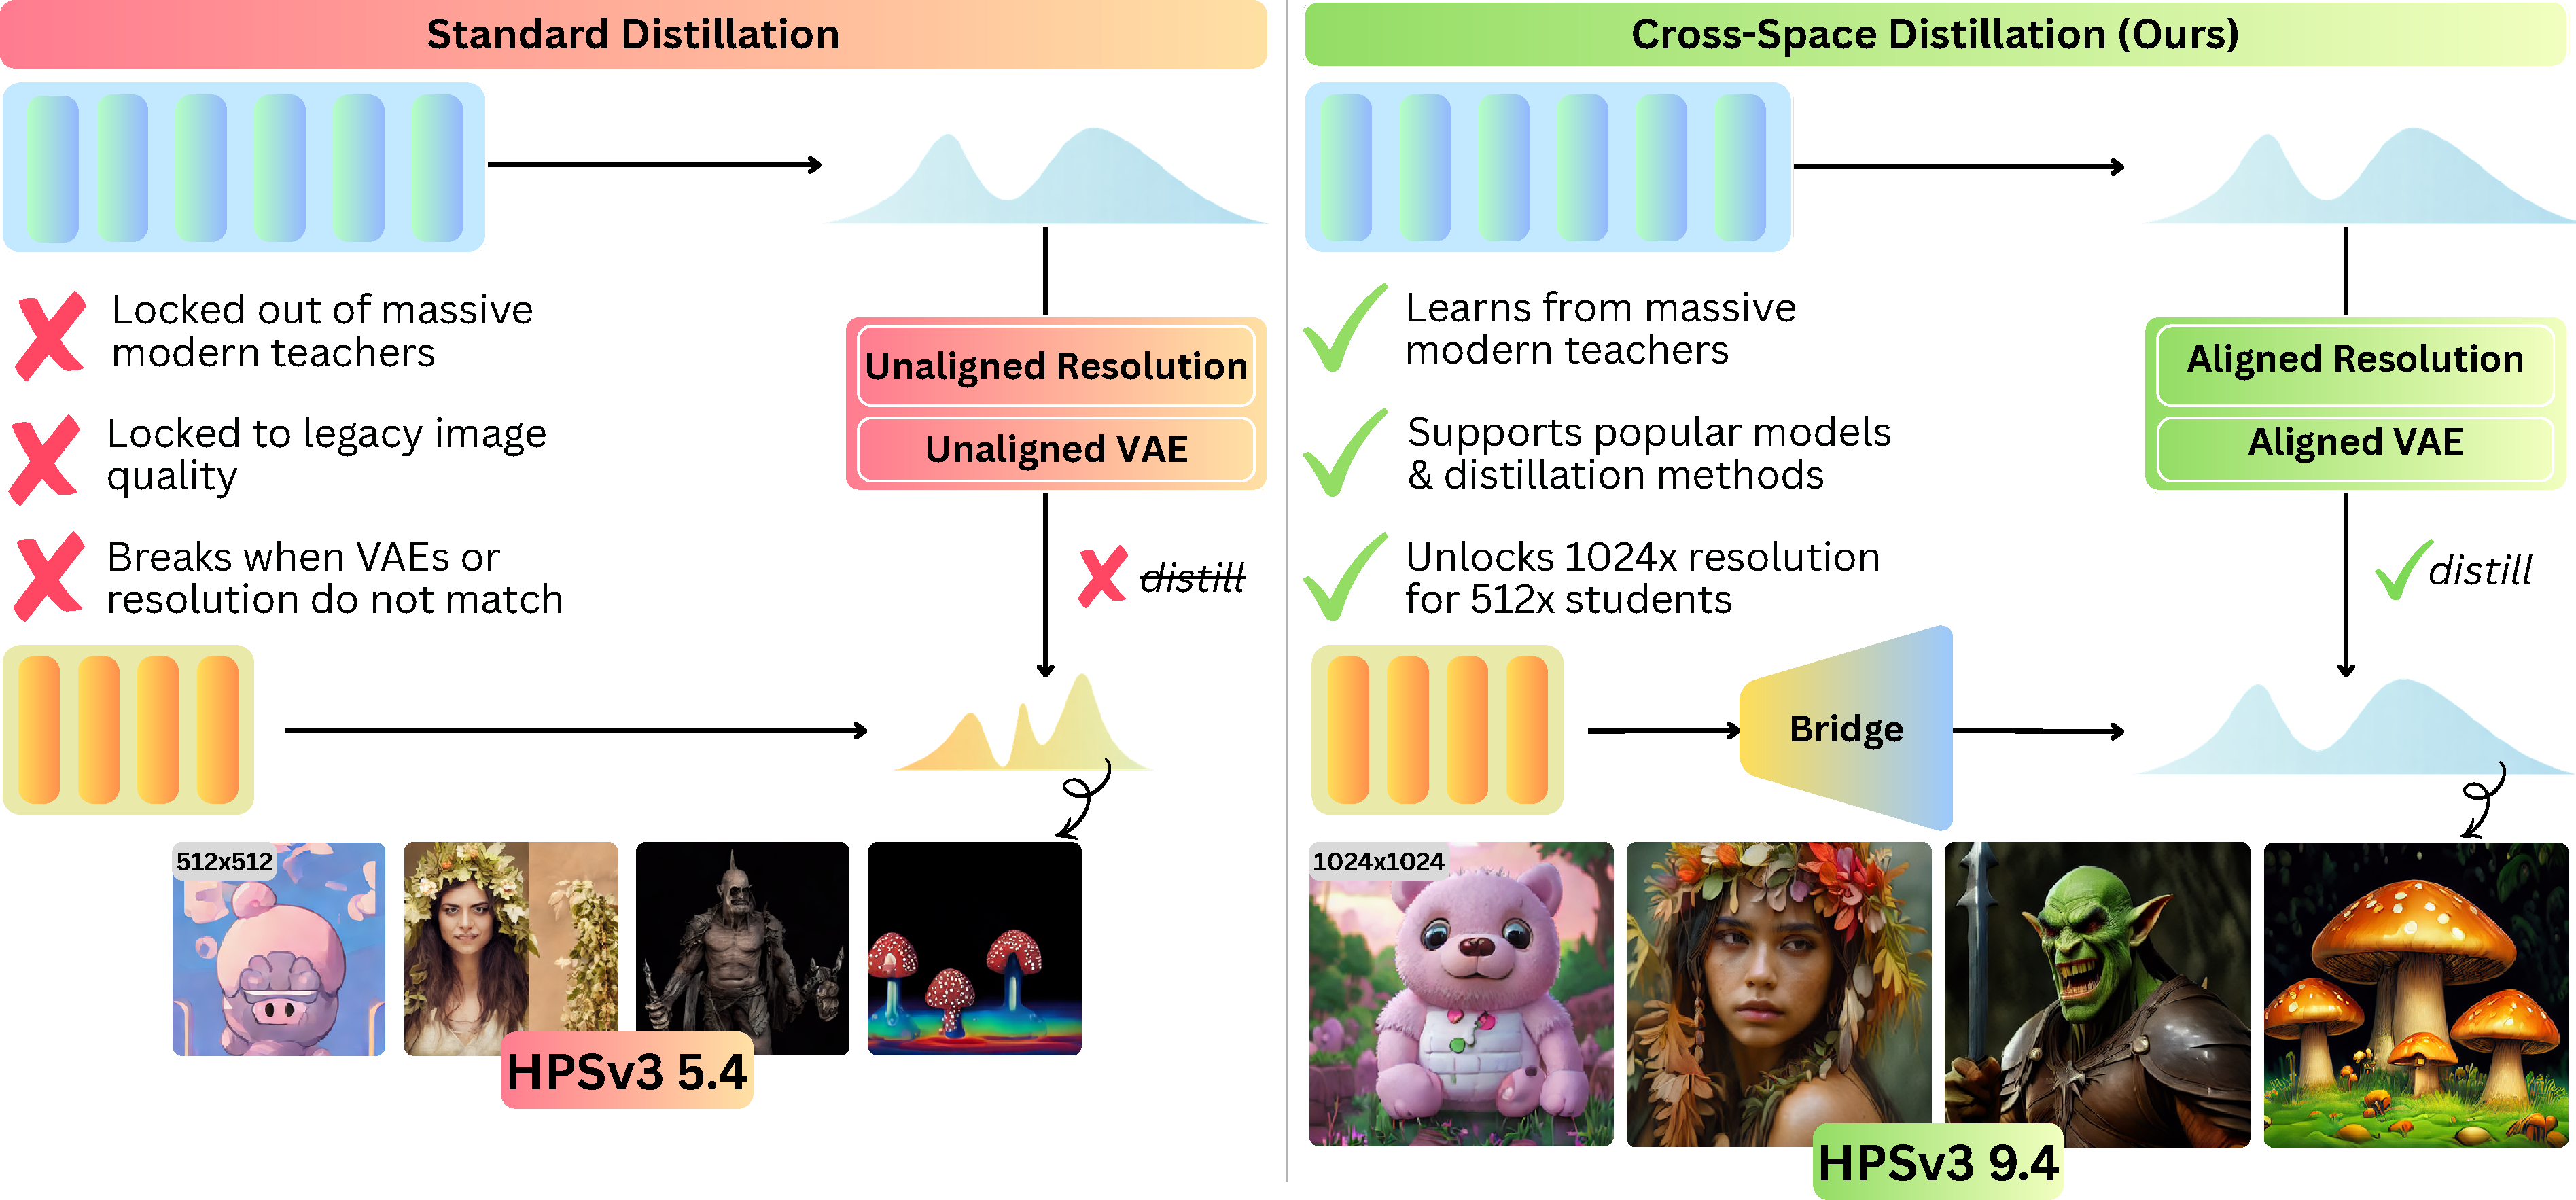
\includegraphics[width=\linewidth]{figures/cross_space_distillation/teaser.pdf}
\caption{Shared-Space vs.\ Cross-Space. Existing distribution distillation assumes a
shared latent; Bridge $\Bridge_\phi$ maps $z_S\mapsto\hat z_T$ so standard one-step
objectives apply without changing the Student backbone.
(Figure from arXiv:2606.32020 source \texttt{assets/teaser.pdf}.)}
\label{fig:teaser}
\end{figure}

%% ============================================================
\section{Bridge construction}
\label{sec:bridge}
%% ============================================================

\textbf{Object.} A frozen (after training) map
\begin{equation}
\hat z_T \;=\; \Bridge_\phi(z_S)
\;\in\; \Za,
\label{eq:bridge-def}
\end{equation}
so Student outputs become Teacher-compatible.

\textbf{Architecture (spatial prior $+$ projector).}
Rather than learning a latent upsampler from scratch, they freeze the first $n$ blocks
of the Student decoder $\Dec_S^{(n)}$ (experiments: $n{=}1$) as a \emph{spatial prior}
that expands the Student grid to the Teacher resolution, then train only a compact
projector $g_\phi$ (SwinIR, ${\sim}5$M params):
\begin{align}
f_{\mathrm{prior}}
&= \Dec_S^{(n)}(z_S)
\in\R^{H\times W\times C_{\mathrm{prior}}},
\label{eq:prior}\\
\hat z_T
&= \Bridge_\phi(z_S)
= g_\phi(f_{\mathrm{prior}})
\in\R^{H\times W\times C_T}.
\label{eq:proj}
\end{align}
Pipeline: $z_S \xrightarrow{\Dec_S^{(n)}} f_{\mathrm{prior}} \xrightarrow{g_\phi} \hat z_T$.

\textbf{Training objectives (offline, paired images).}
Encode the same image with both VAEs to get $(z_S,z_T)$. Minimize
\begin{align}
\mathcal{L}_{\mathrm{rec}}
&= \norm{z_T - \hat z_T}_1,
\label{eq:lrec}\\
\mathcal{L}_{\mathrm{attn}}
&= \sum_{l\in\mathrm{Layers}}
\tau^2\,
\KL\!\big(
P^l(\hat z_T;t,c)
\,\big\|\,
P^l(z_T;t,c)
\big),
\label{eq:lattn}\\
\mathcal{L}_{\mathrm{final}}
&= \alpha\,\mathcal{L}_{\mathrm{rec}} + \beta\,\mathcal{L}_{\mathrm{attn}},
\label{eq:lfinal}
\end{align}
with $\alpha{=}\beta{=}1$, attention temperature $\tau{=}3$, and noising level $t{=}1$ for
attention. $P^l$ are Teacher self-attention row-softmax maps; reverse KL follows MiniLLM
(emphasize dominant mass). Ablations: $\ell_1$ alone is over-smooth; E-LatentLPIPS helps
little; Attention Fidelity restores fine structure (eyes, fur, edges).

\begin{figure}[t]
\centering
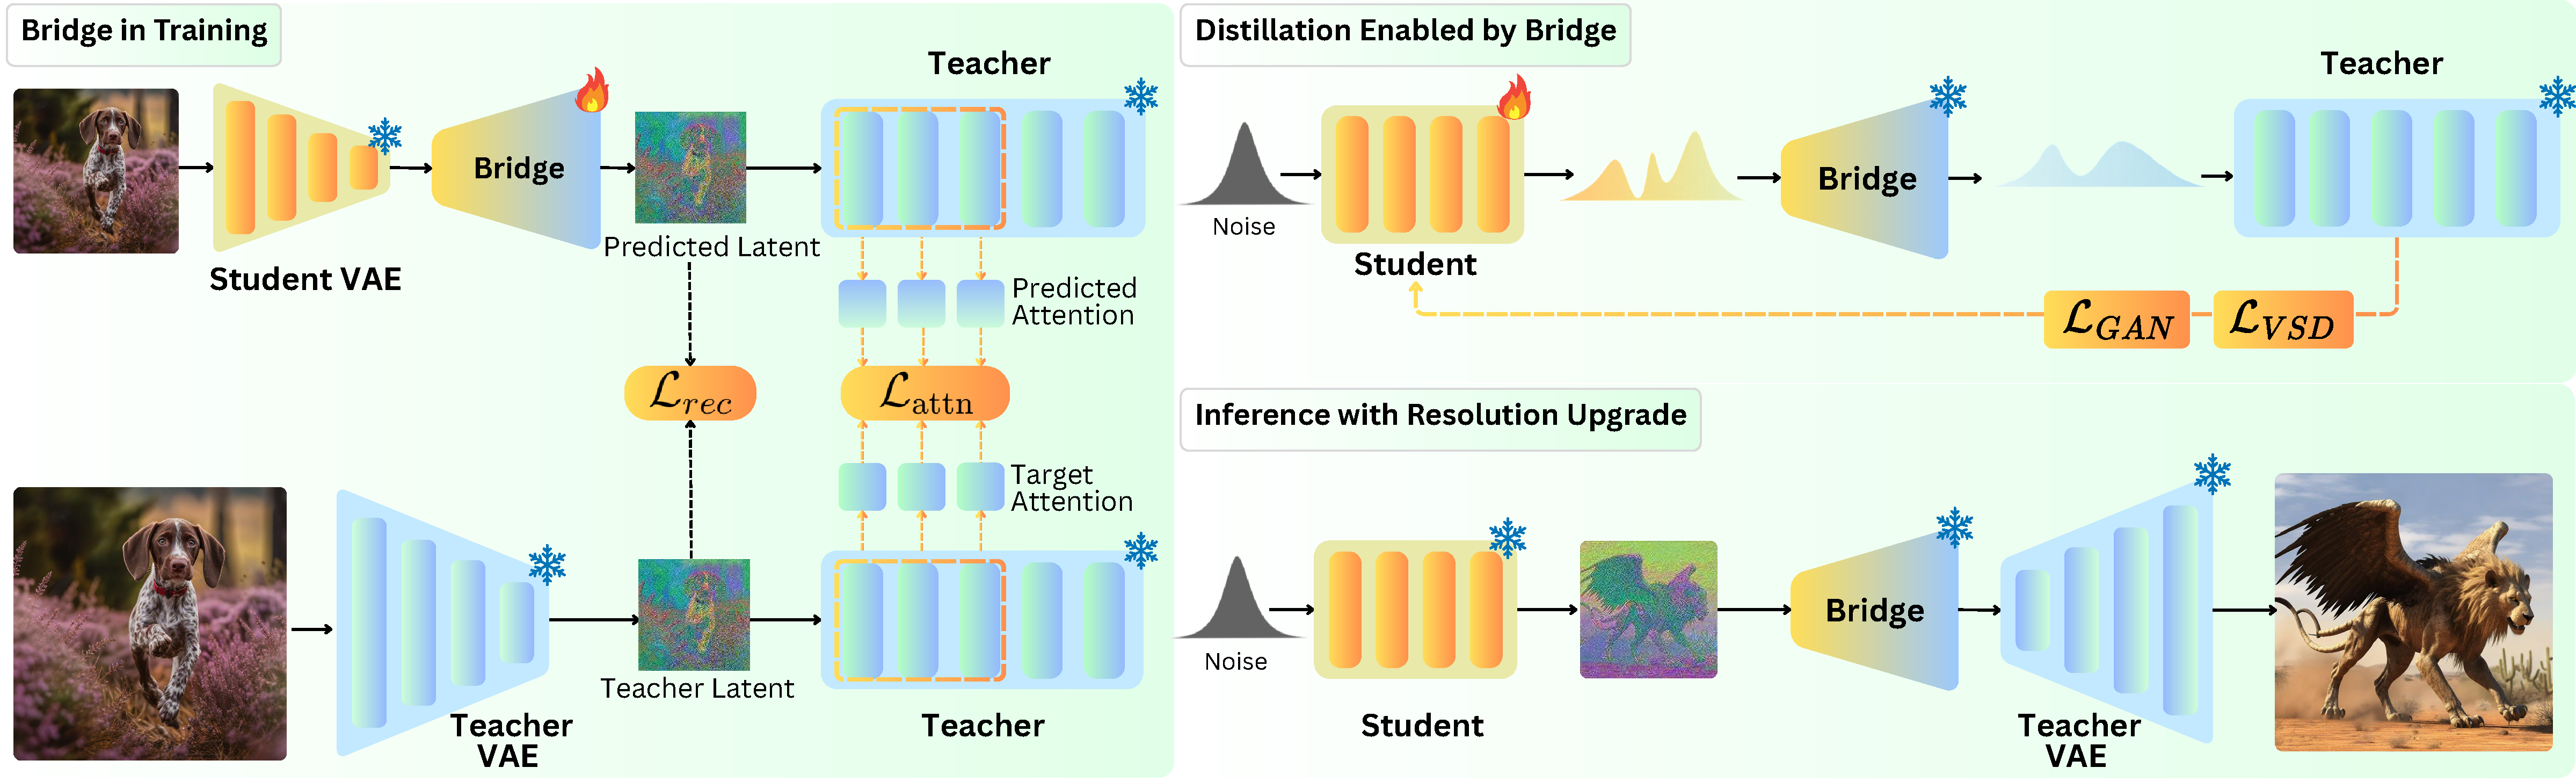
\includegraphics[width=\linewidth]{figures/cross_space_distillation/system.pdf}
\caption{Left: Bridge training with $\mathcal{L}_{\mathrm{rec}}+\mathcal{L}_{\mathrm{attn}}$.
Top-right: freeze Bridge, run VSD/GAN in Teacher space.
Bottom-right: optional inference upgrade --- decode $\hat z_T$ with Teacher decoder at
Teacher resolution.
(Figure from arXiv:2606.32020 source \texttt{assets/system.pdf}.)}
\label{fig:system}
\end{figure}

\begin{figure}[t]
\centering
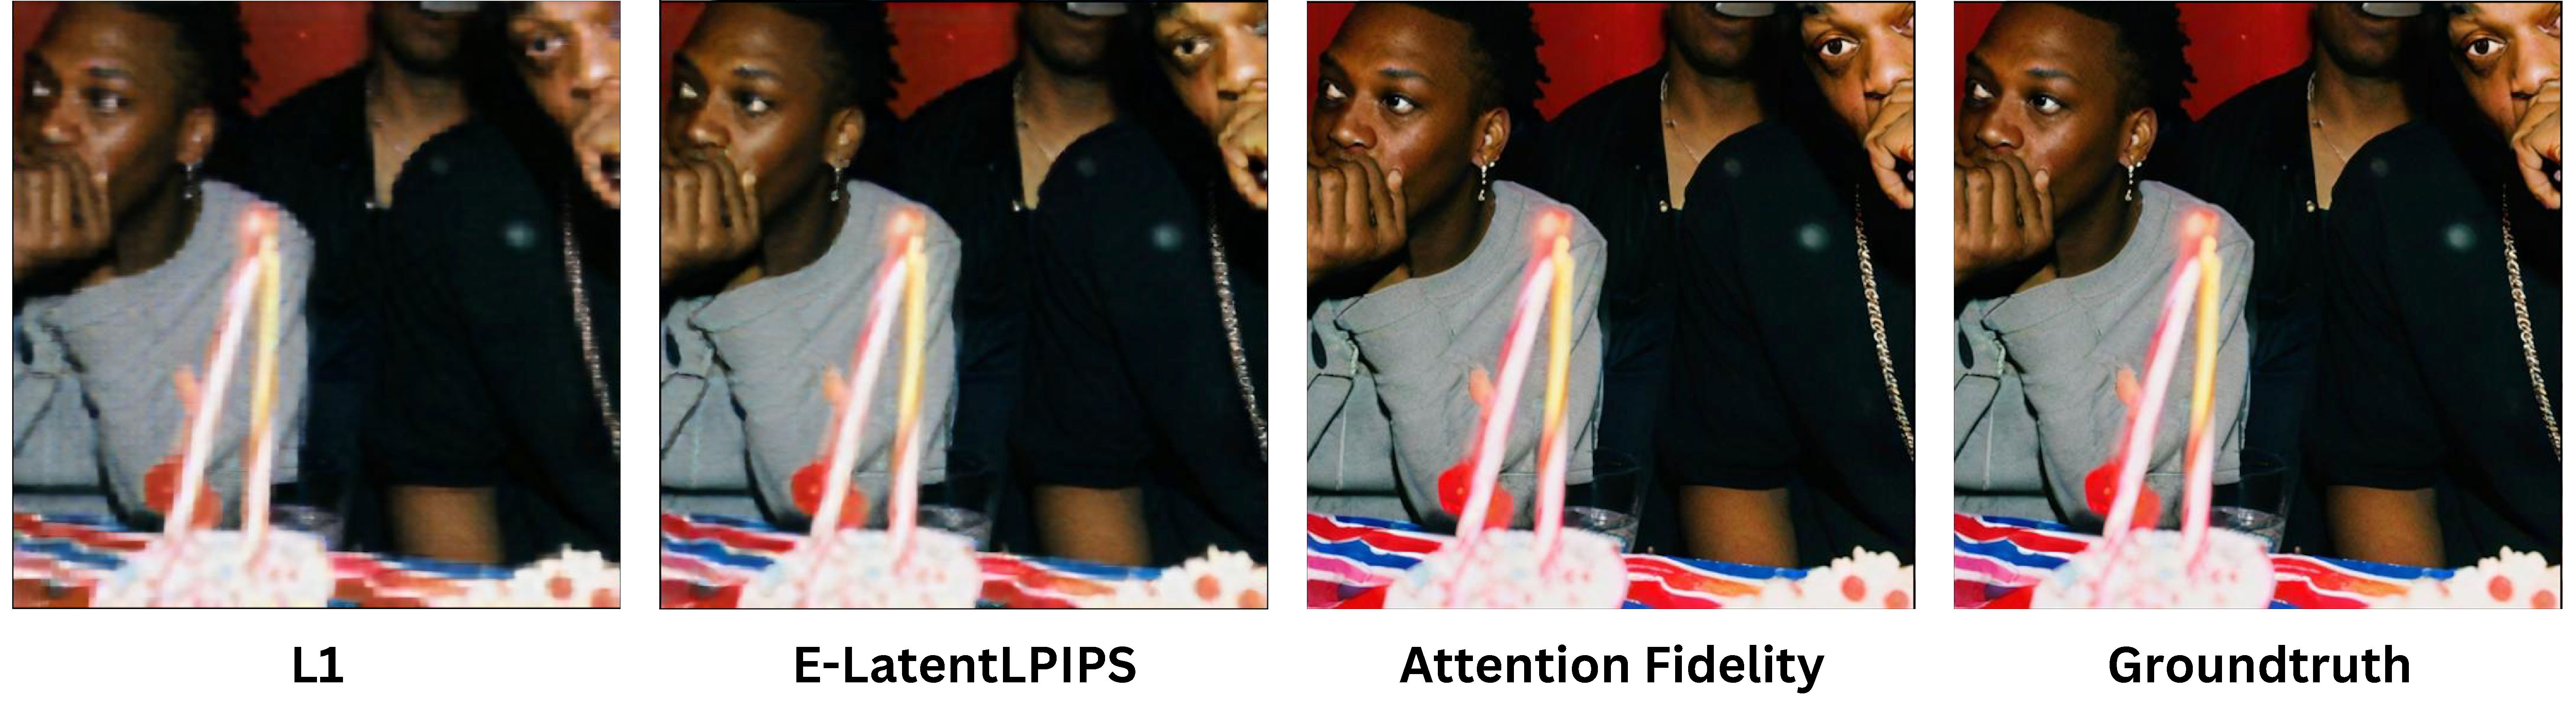
\includegraphics[width=0.95\linewidth]{figures/cross_space_distillation/loss.pdf}
\caption{Objective ablation (SD~2.1$\to$SDXL Bridge): $\ell_1$ only / $+$E-LatentLPIPS /
$+$Attention Fidelity vs.\ GT decode.
(Figure from arXiv:2606.32020 source \texttt{assets/loss.pdf}.)}
\label{fig:loss}
\end{figure}

\textbf{Usage after Bridge is frozen.}
\begin{itemize}[leftmargin=1.4em,itemsep=2pt]
  \item \textbf{Distillation:} Student generates $z_S$; map $\hat z_T=\Bridge_\phi(z_S)$;
        apply DMD2-style $\mathcal{L}_{\mathrm{VSD}}+\mathcal{L}_{\mathrm{GAN}}$ in Teacher
        space (Teacher score / discriminator see $\hat z_T$).
  \item \textbf{Inference upgrade (optional):} same Bridge $+$ Teacher decoder yields
        $1024^2$ outputs from a $512^2$ Student without changing the denoiser.
\end{itemize}

%% ============================================================
\section{Reported evidence (for our design priors)}
\label{sec:evidence}
%% ============================================================

Students: one-step SD~1.5 (DMD2 init) and SD~2.1 (SiD). Teachers: SDXL, Kolors,
PixArt-$\Sigma$, FLUX.2-klein-4B, SD~3.5~M (all $1024^2$). Bridge trained on ${\sim}2$M
Teacher-synthesized images (JourneyDB/LAION prompts). Headline: SD~1.5 HPSv3
$5.37\to 9.42$ (SD~3.5~M teacher), merged average of five distilled students reaches
$10.53$. Mechanism-agnostic $x_0$ reparameterization enables flow Teachers $\to$ DDPM
Students without layer-wise matching.

%% ============================================================
\section{Map onto XOPD notation}
\label{sec:map}
%% ============================================================

Recall our notation (\texttt{cross\_latent\_distillation\_problem.tex}):
forward $\Tmap:\Za\to\Zb$ (teacher$\to$student, easy when $d_T>d_S$),
inverse $\Tinv:\Zb\to\Za$ (hard). Ideal on-manifold lift
$\bar z_T(z_S)=\Enc_T(\Dec_S(z_S))$.

\begin{observation}[Bridge is a learned inverse $Q$, not a forward $\Tmap$]
\label{obs:bridge-is-Q}
$\Bridge_\phi:\Zb\to\Za$ is exactly the student$\to$teacher direction we call $Q$ /
$\Tinv$. The frozen $\Dec_S^{(n)}$ is an architectural prior for \emph{spatial}
expansion; $g_\phi$ does channel/semantic alignment. Training pairs are
$(z_S,z_T)=(\Enc_S(x),\Enc_T(x))$, so the regression target is the
\textbf{pixel-anchored} Teacher encode --- the same ideal lift
$\bar z_T$ that our notes treat as the on-manifold gold standard --- plus an
attention regularizer in Teacher space.
\end{observation}

\begin{table}[h]
\centering
\small
\begin{tabular}{@{}p{3.2cm}p{4.6cm}p{4.6cm}@{}}
\toprule
& \textbf{Cross-Space Bridge} & \textbf{XOPD cross-VAE (ours)} \\
\midrule
Primary mismatch & Cross-Res.\ $+$ Cross-VAE & Cross-VAE (often also Res.) \\
Hard map learned & $Q=\Bridge_\phi:\Zb\to\Za$ & $Q$ (HSCT / disc.\ / cINN / \ldots) \\
Easy map & unused during distill (Student stays in $\Zb$) &
  linear $P:\Za\to\Zb$ for L0 / pushforward \\
Distill objective & VSD / GAN on $\hat z_T$ (measure matching) &
  L0 sample transport $+$ L1 transition / velocity in $\Zb$ \\
Where Teacher is queried & Teacher space after Bridge &
  either Teacher space via $Q$, or Student space via $P\push$ \\
Spatial prior & frozen $\Dec_S^{(n)}$ &
  optional; often pixel bridge $\Enc_T(\Dec_S(\cdot))$ \\
Extra supervision & reverse-KL on Teacher attention &
  cycle / adv / NLL / hidden-state cond.\ (HSCT) \\
\bottomrule
\end{tabular}
\caption{Bridge vs.\ XOPD cross-VAE: same hard inverse direction, different distill
geometry.}
\label{tab:compare}
\end{table}

\begin{remark}[Why this is Route~A-adjacent, not L1 pushforward]
\label{rem:route-a}
\texttt{avoid\_inverse\_transport\_analysis.tex} Route~A replaces pointwise velocity
targets by score / DMD-style measure matching so that supervision lives where the
Teacher is defined --- after a push of Student samples into Teacher space (or a shared
score space). Bridge is precisely the missing interface that makes Route~A
\emph{implementable} under Cross-VAE: freeze $Q=\Bridge_\phi$, then run DMD2 in
$\Za$. It does \textbf{not} construct a differentiable forward $\Tmap$ with Jacobian
for $(\Tmap\push v_T)$ in Student coordinates; therefore it does not by itself make
XOPD L1 (pointwise transition matching in $\Zb$) well-posed.
\end{remark}

\begin{remark}[Relation to methods already in our inverse note]
\label{rem:vs-methods}
\begin{itemize}[leftmargin=1.4em,itemsep=2pt]
  \item vs.\ \textbf{pixel bridge} $\Enc_T(\Dec_S(z_S))$: Bridge keeps a frozen decoder
        \emph{prefix} (cheaper than full decode) and replaces the Teacher encode by a
        learned $g_\phi$ supervised with $\ell_1$ $+$ attention --- a trainable
        refinement of the same on-manifold idea.
  \item vs.\ \textbf{MSE / linear $Q$}: paper confirms $\ell_2$/mean-seeking is weak;
        they use $\ell_1$ and add Teacher-attention reverse KL instead of a latent
        discriminator (Method~1) or cINN (Method~2).
  \item vs.\ \textbf{HSCT / M8}: HSCT conditions $Q$ on student DiT hidden states for
        on-policy L1 queries; Bridge is offline, prompt/image-paired, and
        \emph{does not} use student transformer features --- it relies on VAE spatial
        prior $+$ Teacher attention.
  \item vs.\ \textbf{same-VAE DMD} (\texttt{dmd\_cross\_model\_design.md}): that RFC
        assumes shared VAE. Under Cross-VAE, Bridge (or equivalent $Q$) is a
        prerequisite before real/fake scores can share a latent.
\end{itemize}
\end{remark}

\begin{tcolorbox}[colback=blue!4,colframe=blue!50!black,title=Takeaway for Flow-Factory XOPD]
If the goal is \textbf{cross-VAE one-step / DMD-style} distillation into a compact
backbone: Bridge is a strong external recipe for learning $Q$ (spatial prior $+$
$\ell_1$ $+$ Attention Fidelity) and then running Teacher-space VSD/GAN --- align with
Route~A, not with linear-$P$ L1.
If the goal remains \textbf{multi-step on-policy OPD with L0/L1 in Student space}:
Bridge alone is insufficient; still need forward $P$ (or pixel adjoint Route~B) for
Student-space losses. Attention Fidelity is a reusable objective to add on top of any
learned $Q$ (disc.\ / HSCT / cINN) to keep $\hat z_T$ Teacher-attention-compatible.
\end{tcolorbox}

\section*{Cross References}
\begin{itemize}[leftmargin=1.4em,itemsep=1pt]
  \item Paper:
        \href{https://arxiv.org/abs/2606.32020}{arXiv:2606.32020}
        (Cross-Space Distillation).
  \item Problem formalization:
        \texttt{docs/xopd/cross\_latent\_distillation\_problem.tex}.
  \item Avoiding the hard inverse / Route~A:
        \texttt{docs/xopd/avoid\_inverse\_transport\_analysis.tex}.
  \item Inverse algorithms (disc.\ / cINN):
        \texttt{docs/xopd/inverse\_mapping\_methods.tex}.
  \item Method zoo (M1--M7):
        \texttt{docs/xopd/xopd\_vae\_space\_align.tex}.
  \item Same-VAE DMD design:
        \texttt{docs/xopd/dmd\_cross\_model\_design.md}.
\end{itemize}

\end{document}
